\startfirstchapter{Results}
\label{chapter:results}

This chapter presents the results of applying the statistical analysis presented in Chapter \ref{chapter:stat} to the MC simulated and observed ATLAS collision events selected for the search\footnote{See Section \ref{sec:evt_selections} for details of the selections applied to define the regions of the search}.  


\section{Background-only Fit}

\subsection{Pre- and Post-Fit Yields of MC Simulated Background Events}

\begin{figure}[!tb]
  \centering
  \begin{subfigure}{0.45\textwidth}
    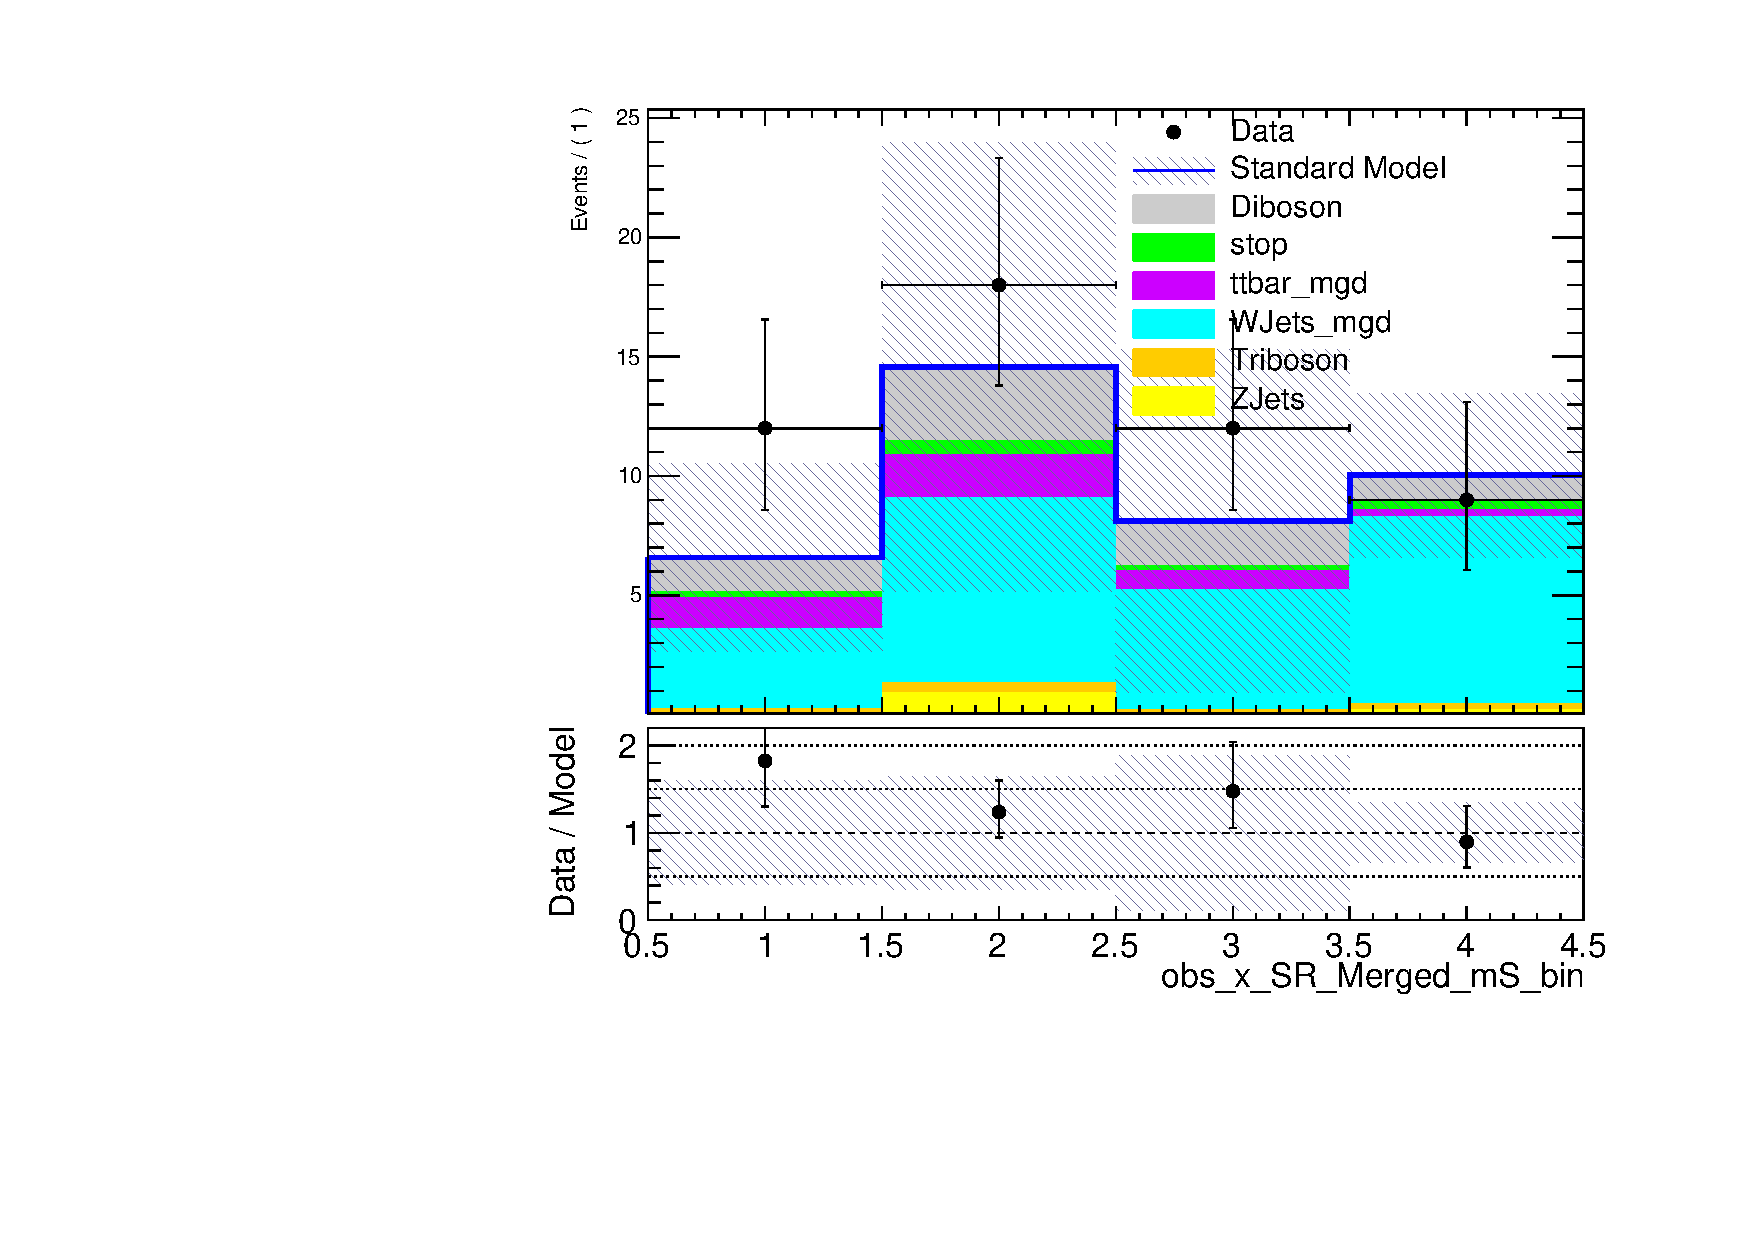
\includegraphics[width=\textwidth]{figures/12_results/BkgOnly/SR_Merged_mS_bin_beforeFit.pdf}
    \caption{\merged SR pre-fit}\label{fig:prefit_merged_SR_bkgonly}
  \end{subfigure} \hspace{1em}
  \begin{subfigure}{0.45\textwidth}
    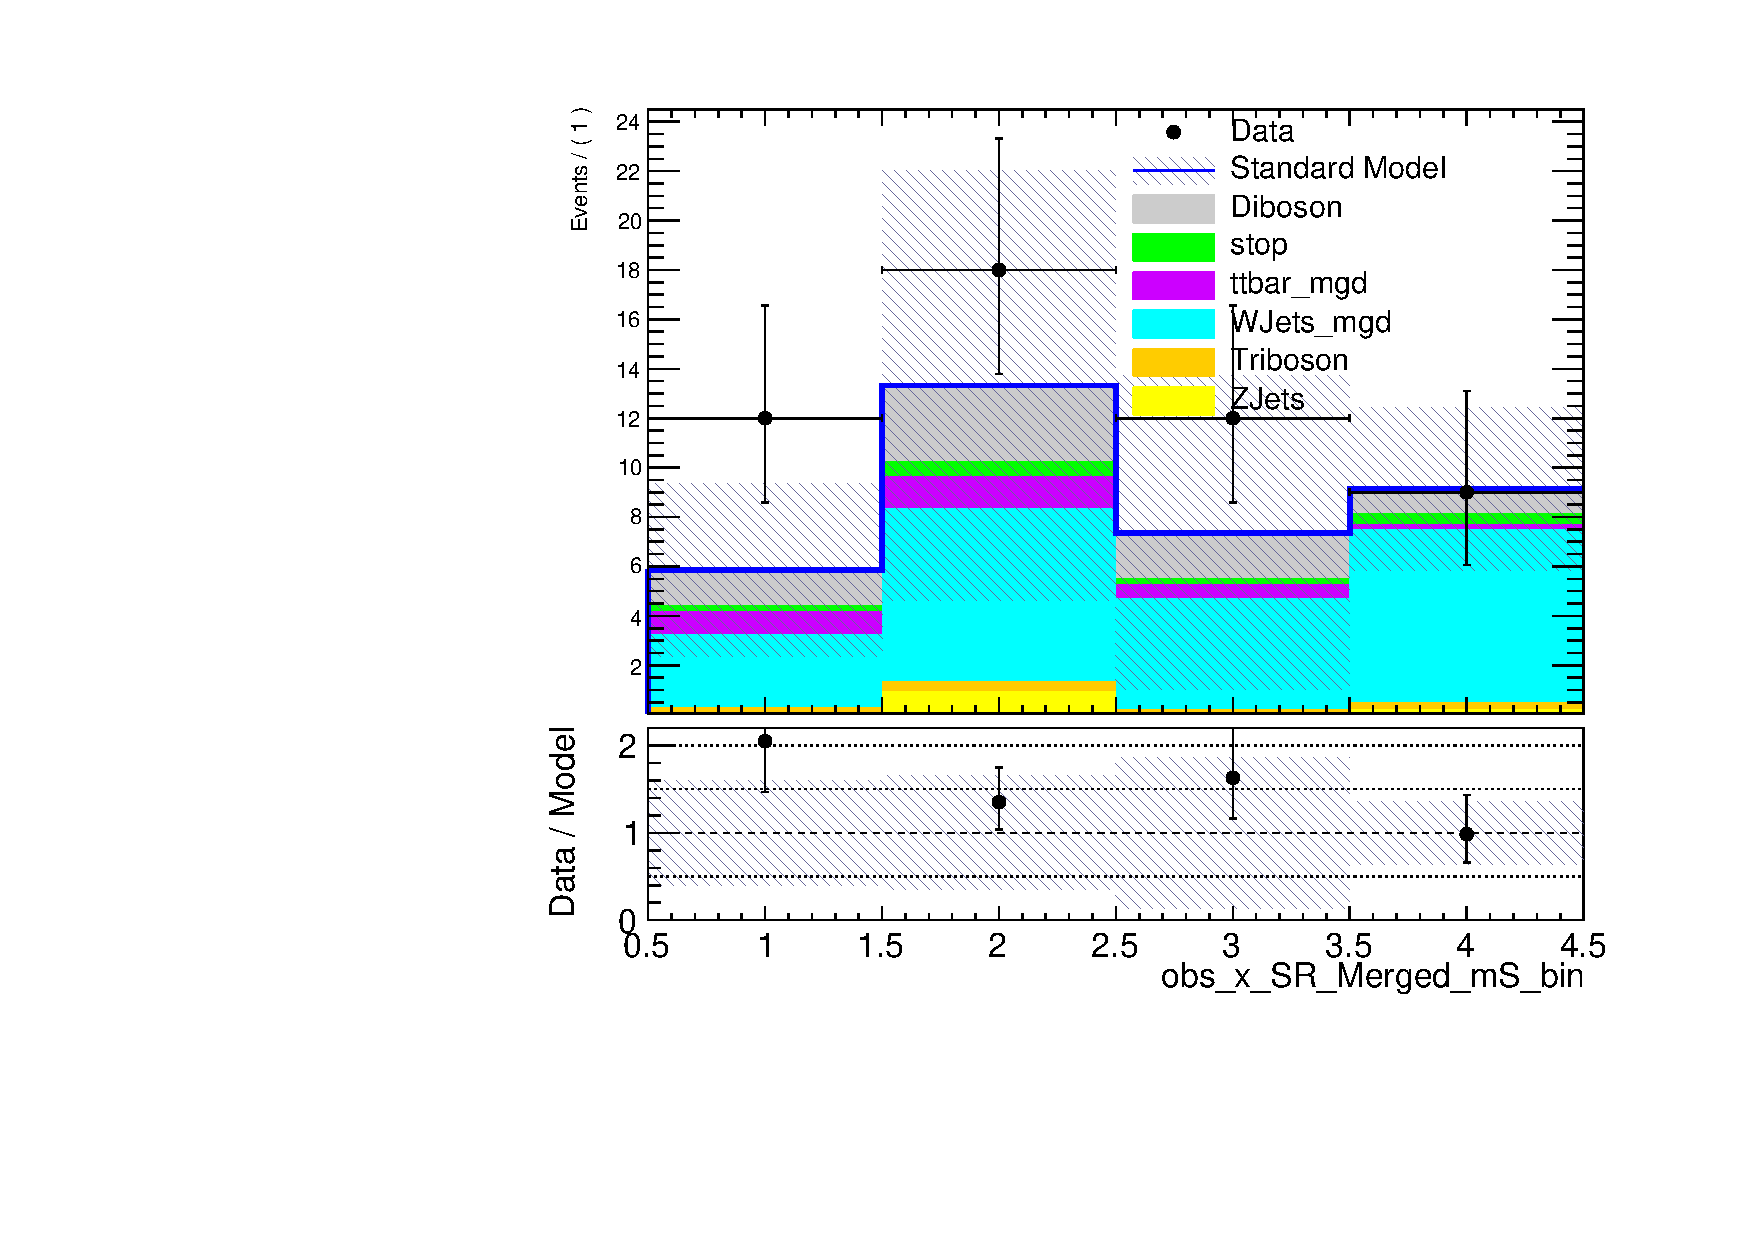
\includegraphics[width=\textwidth]{figures/12_results/BkgOnly/SR_Merged_mS_bin_afterFit.pdf}
    \caption{\merged SR post-fit}\label{fig:postfit_merged_SR_bkgonly}
  \end{subfigure} \\ \vspace{1em}
  \begin{subfigure}{0.45\textwidth}
    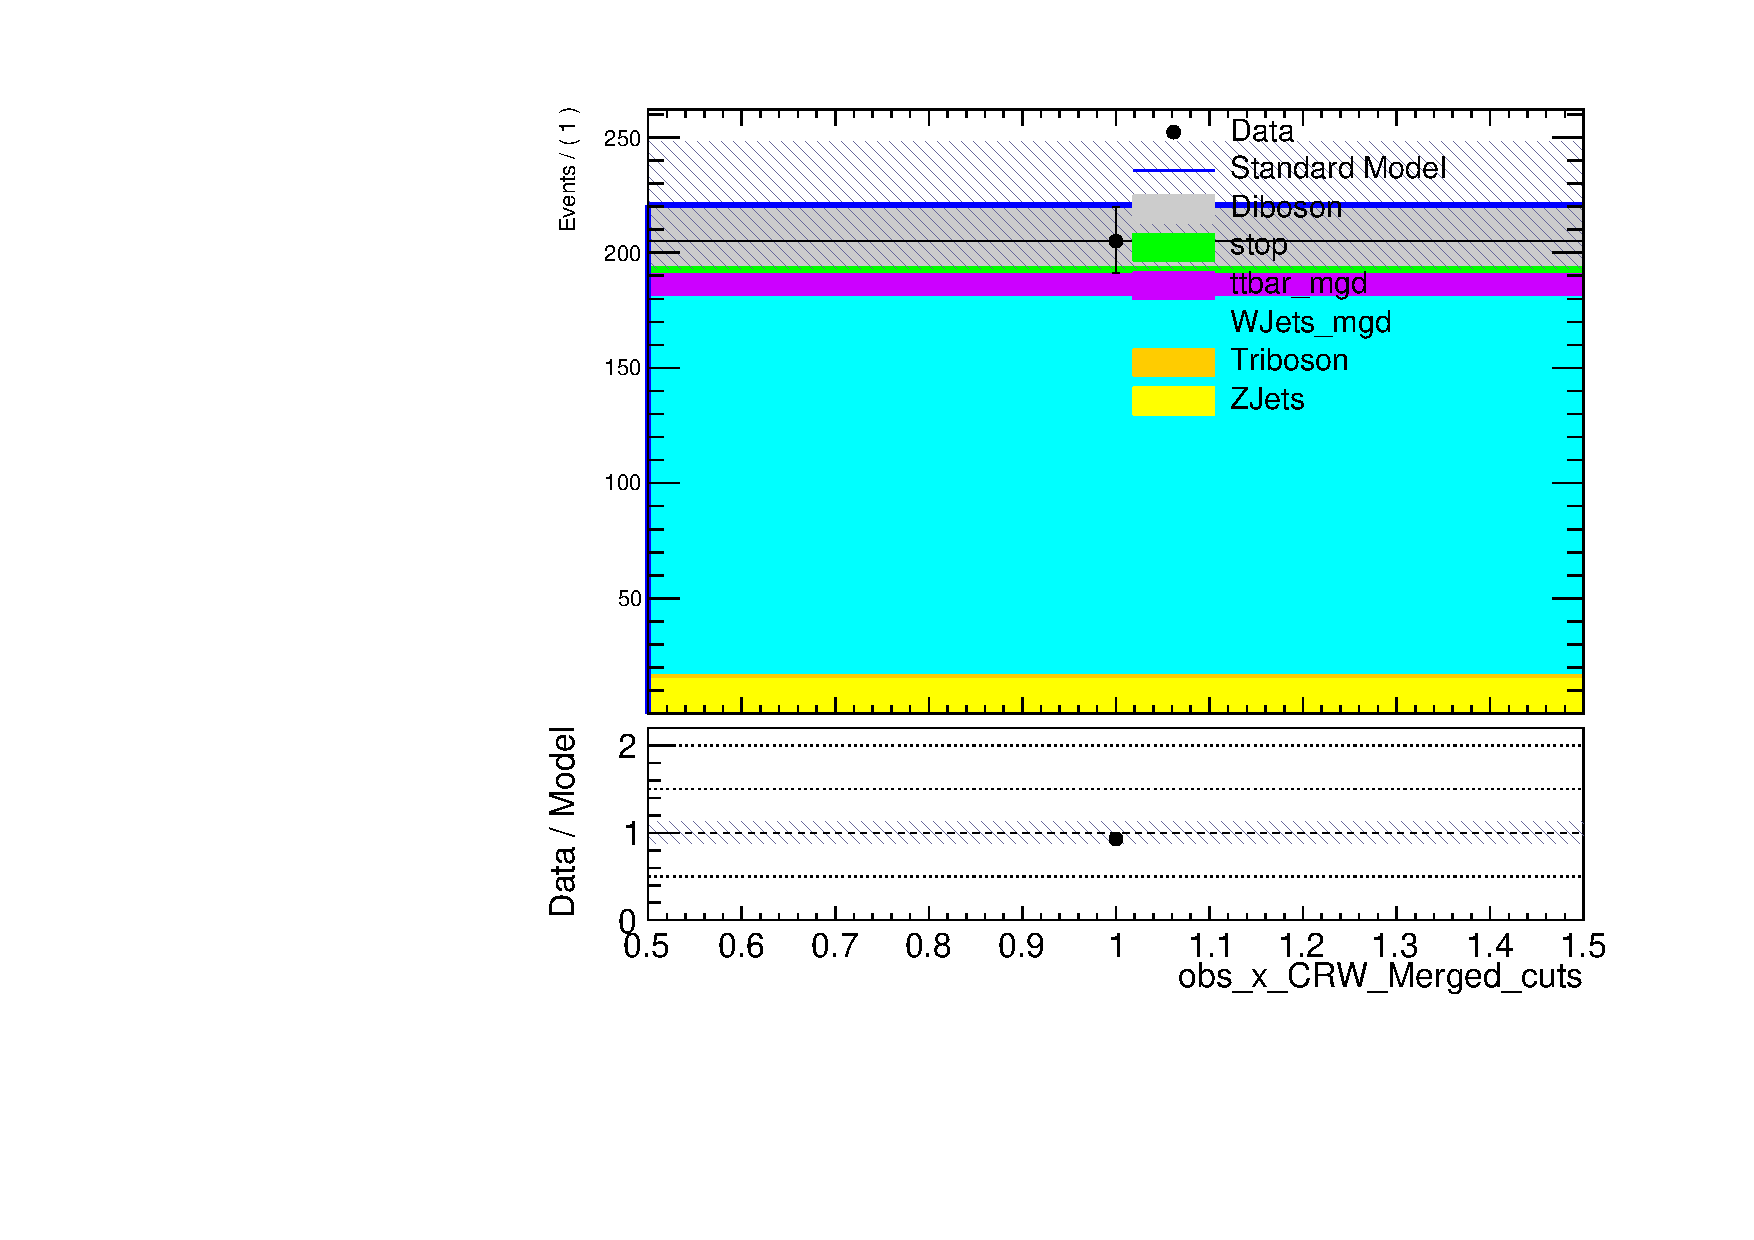
\includegraphics[width=\textwidth]{figures/12_results/BkgOnly/CRW_Merged_cuts_beforeFit.pdf}
    \caption{\merged CRW pre-fit}\label{fig:prefit_merged_CRW_bkgonly}
  \end{subfigure} \hspace{1em}
  \begin{subfigure}{0.45\textwidth}
    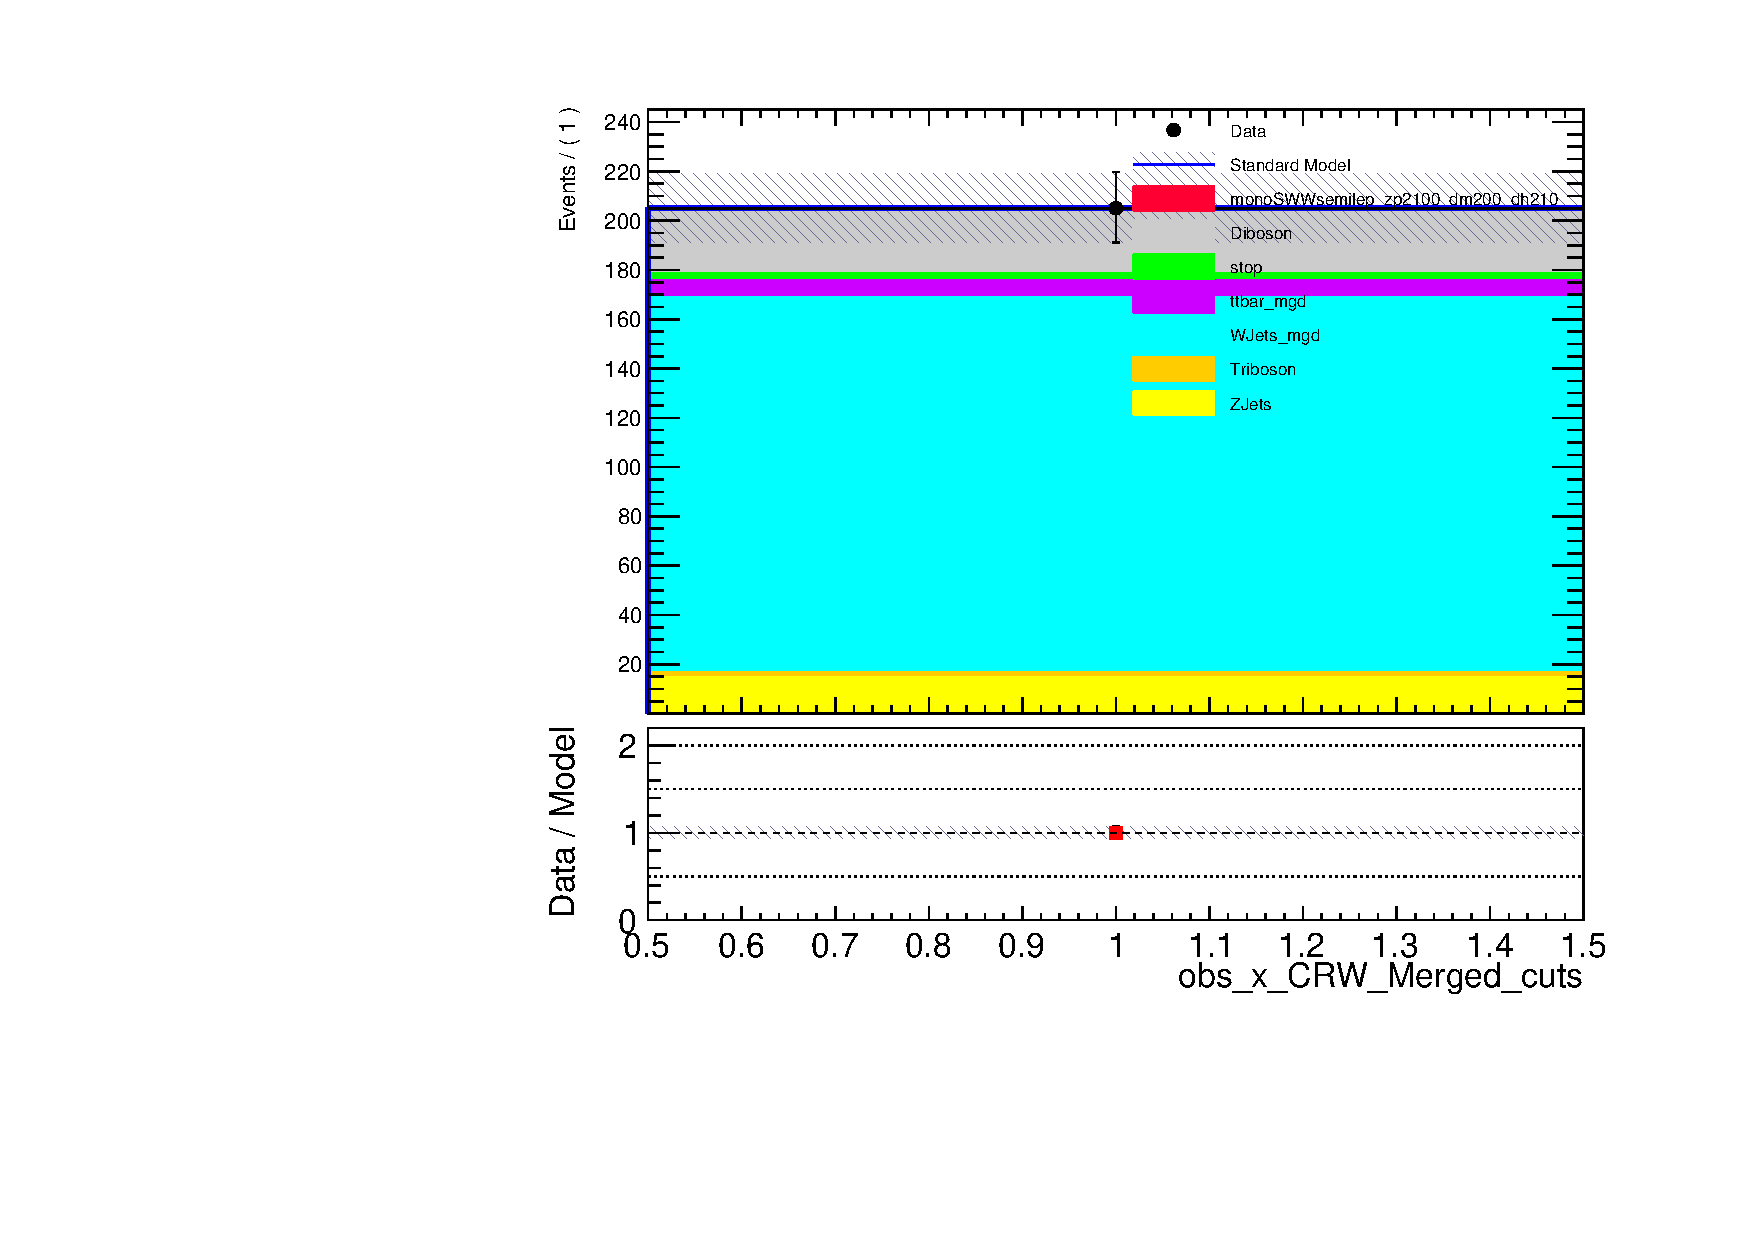
\includegraphics[width=\textwidth]{figures/12_results/BkgOnly/CRW_Merged_cuts_afterFit.pdf}
    \caption{\merged CRW post-fit}\label{fig:postfit_merged_CRW_bkgonly}
  \end{subfigure} \\ \vspace{1em}
    \begin{subfigure}{0.45\textwidth}
    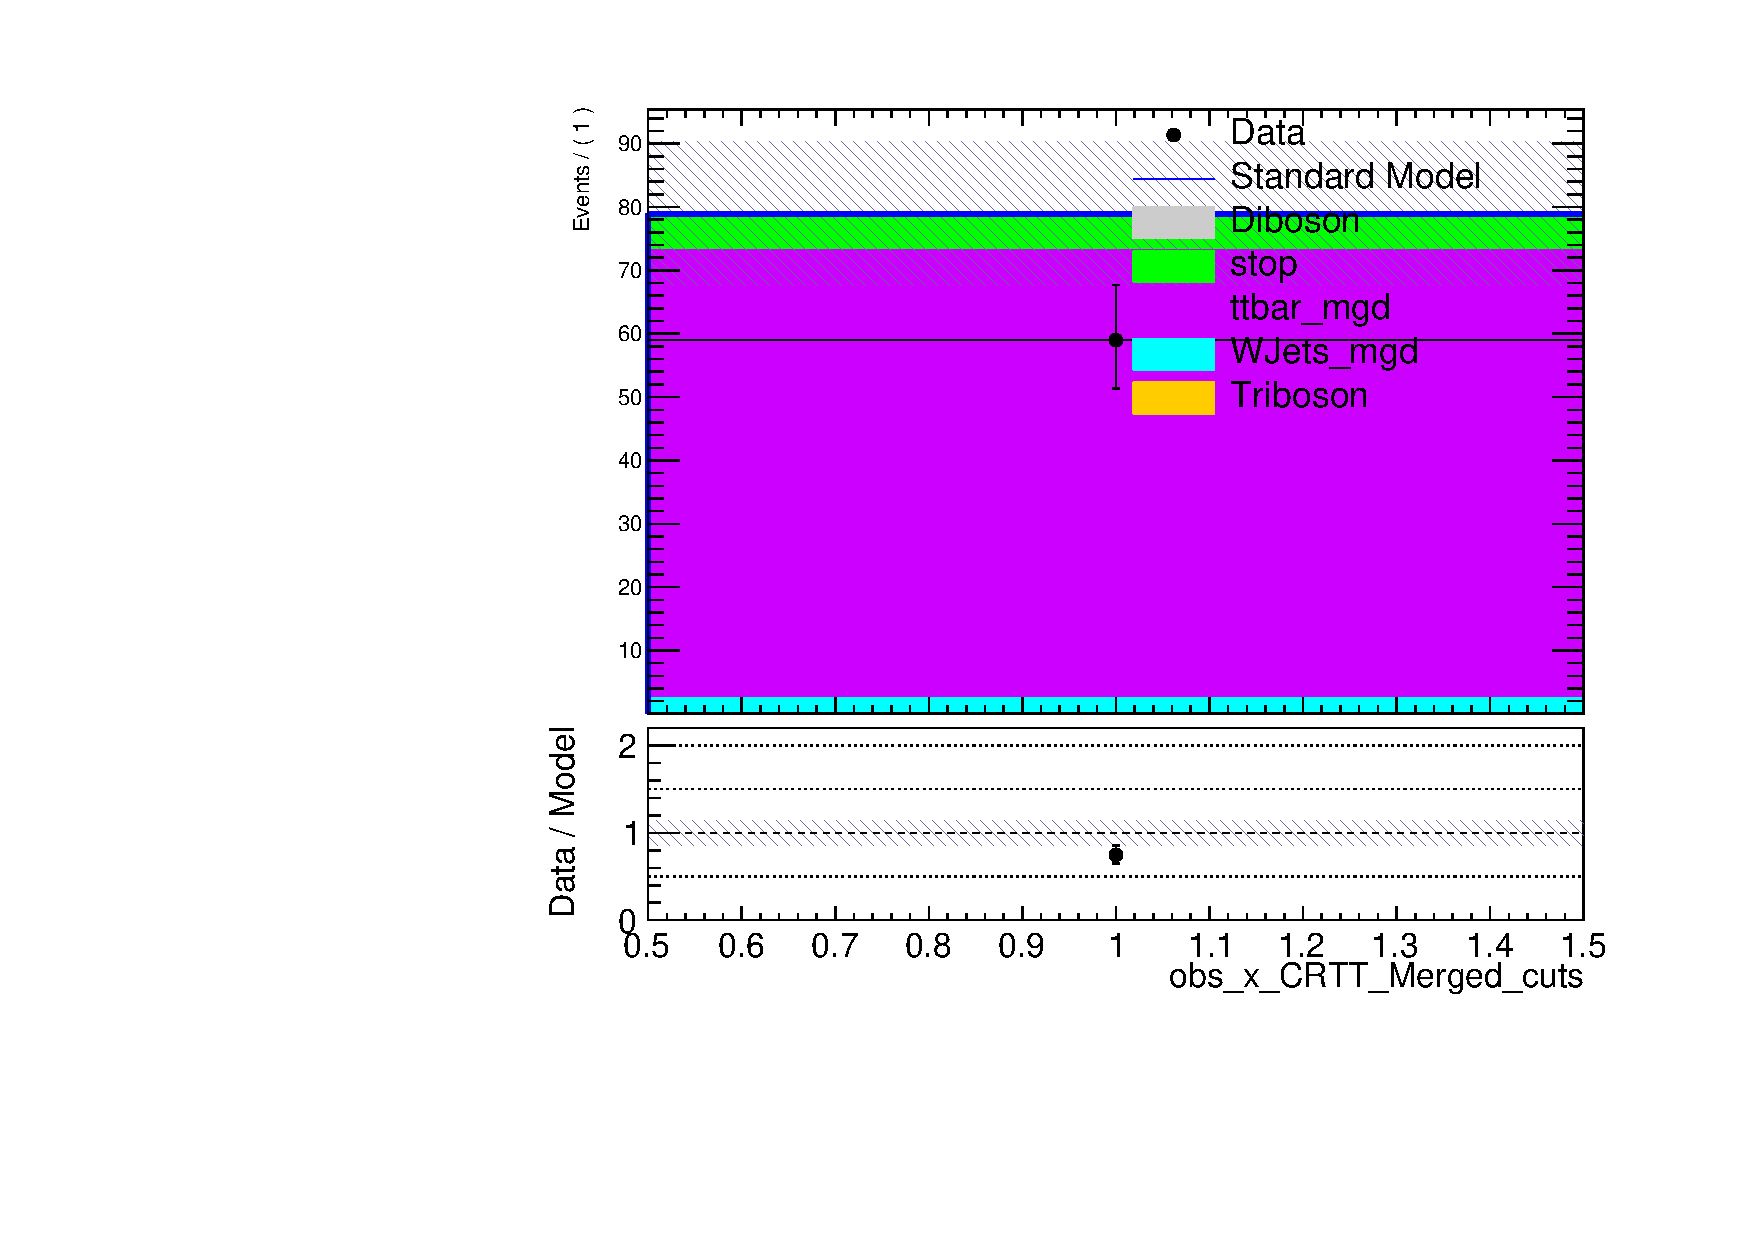
\includegraphics[width=\textwidth]{figures/12_results/BkgOnly/CRTT_Merged_cuts_beforeFit.pdf}
    \caption{\merged CRTT pre-fit}\label{fig:prefit_merged_CRTT_bkgonly}
  \end{subfigure} \hspace{1em}
  \begin{subfigure}{0.45\textwidth}
    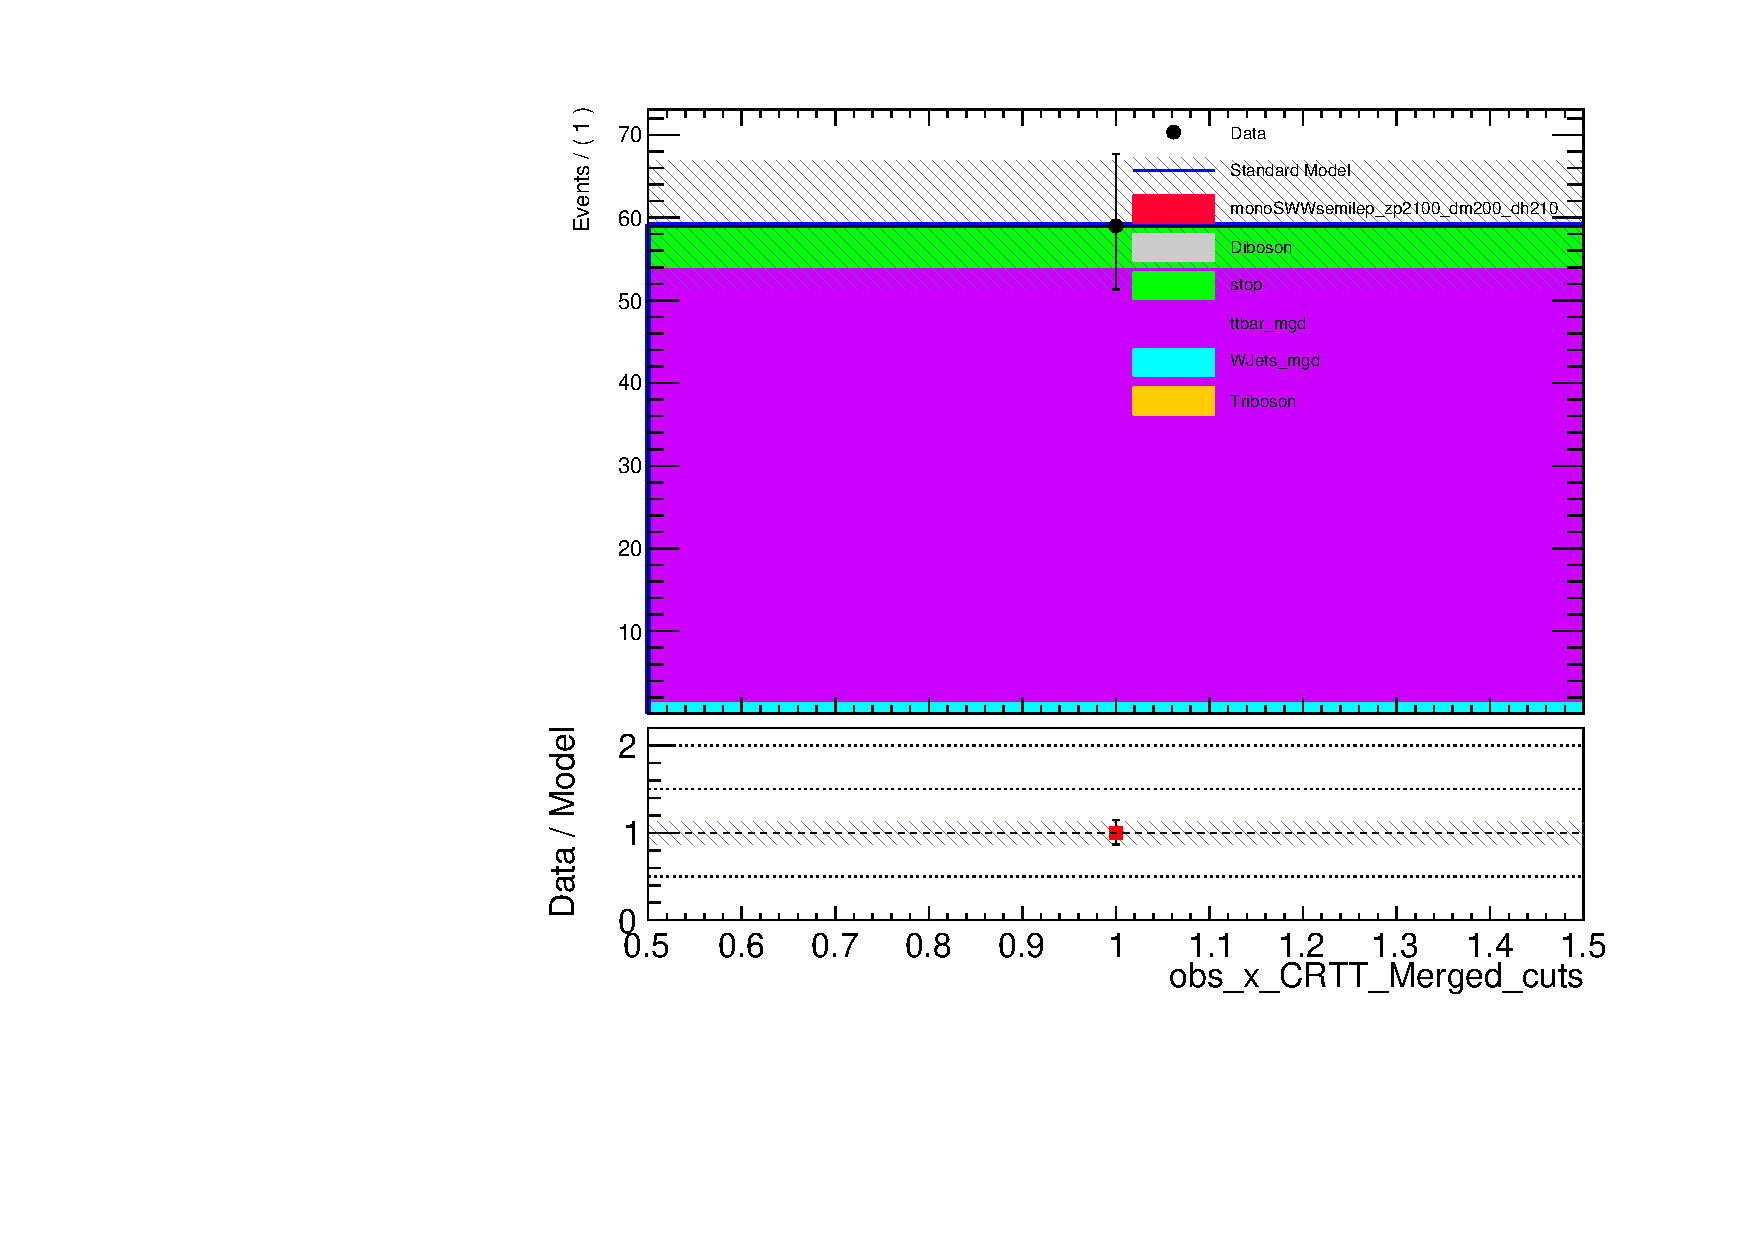
\includegraphics[width=\textwidth]{figures/12_results/BkgOnly/CRTT_Merged_cuts_afterFit.pdf}
    \caption{\merged CRTT post-fit}\label{fig:postfit_merged_CRTT_bkgonly}
  \end{subfigure}
  \caption[Pre- and post-fit distributions in \merged analysis regions for background-only fit]{Pre-fit (left) and post-fit (right) distributions for a background-only fit in the three \merged analysis regions, with the binning used in the HistFitter fit. The Run-2 data set is used in the control regions and Asimov data is used in the signal regions. Background MC is normalized to the data luminosity of \Lumi.}
  \label{fig:pre_post_merged_bkgonly}
\end{figure}

\begin{figure}[!tb]
  \centering
  \begin{subfigure}{0.45\textwidth}
    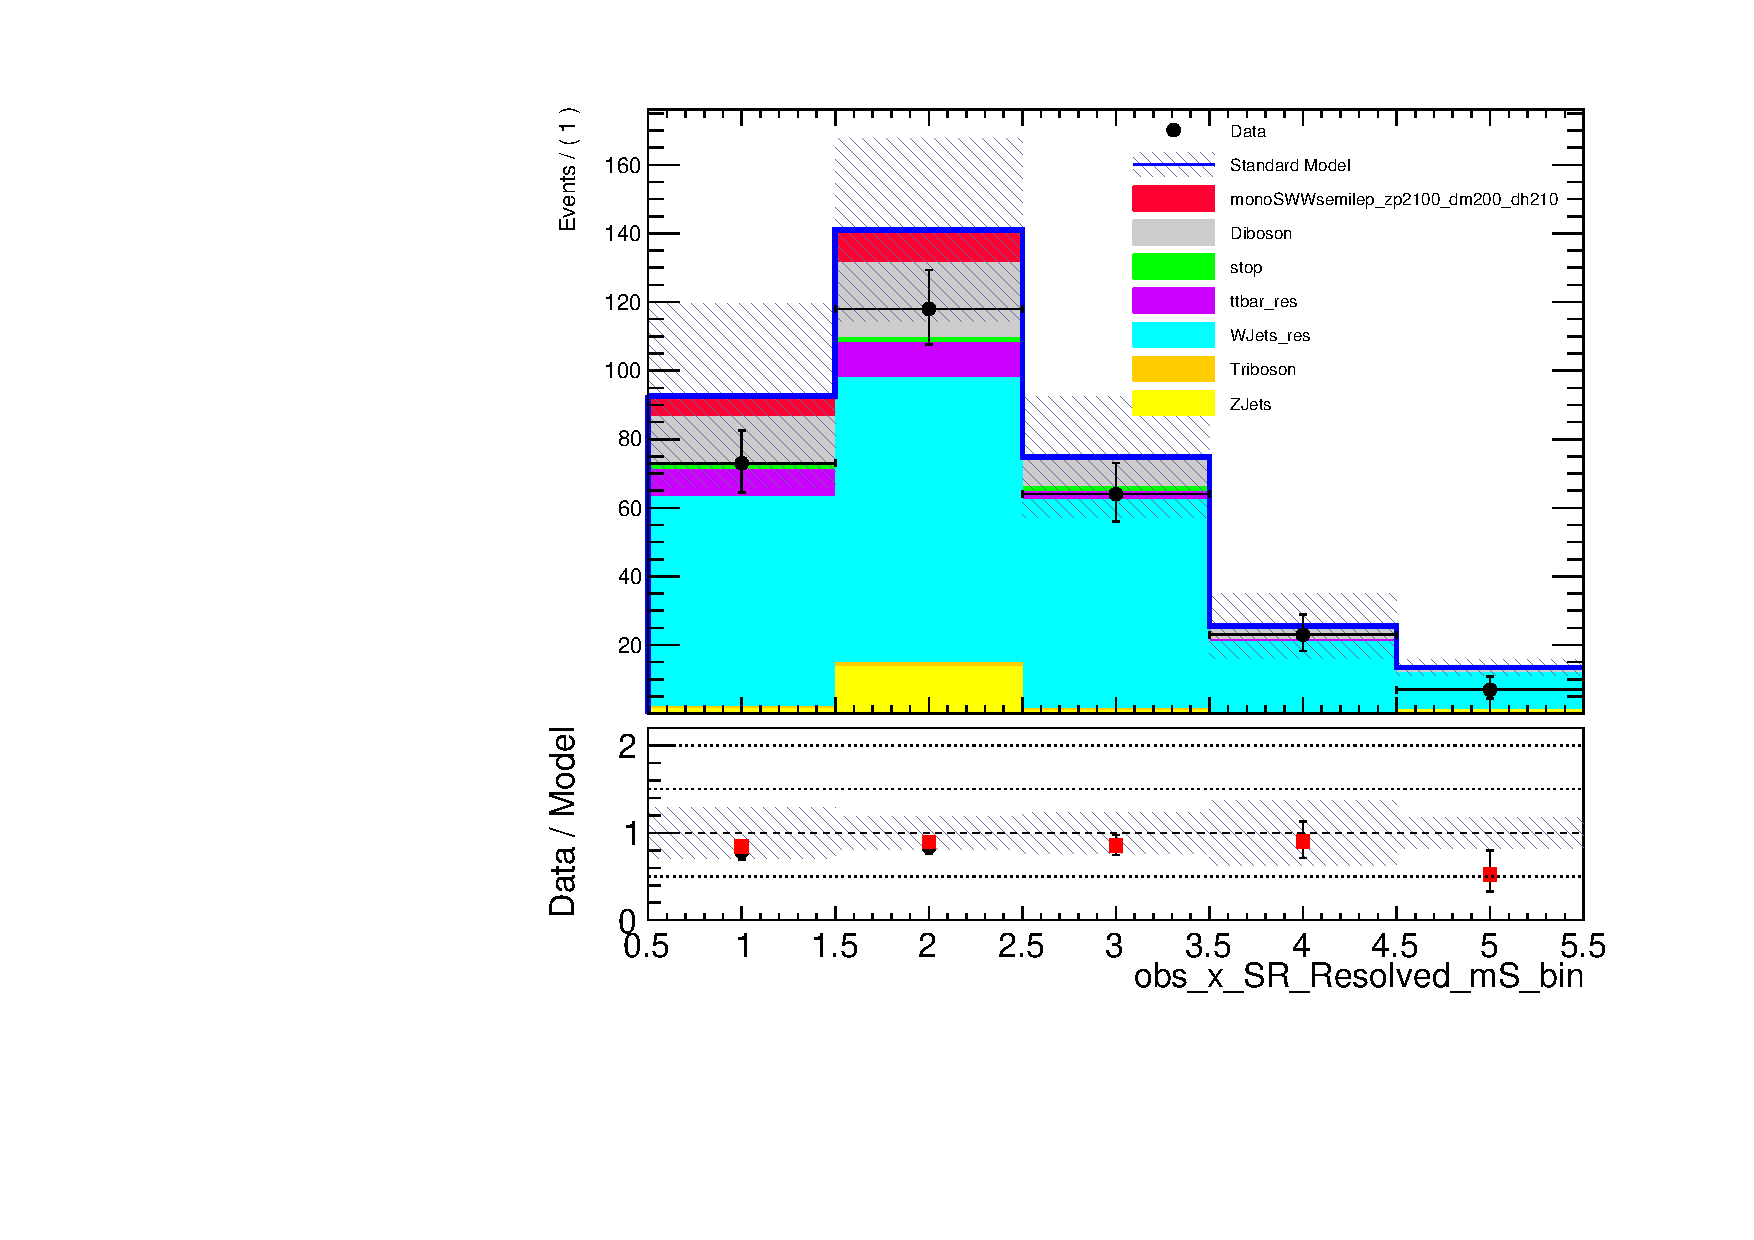
\includegraphics[width=\textwidth]{figures/12_results/BkgOnly/SR_Resolved_mS_bin_beforeFit.pdf}
    \caption{\resolved SR pre-fit}\label{fig:prefit_resolved_SR_bkgonly}
  \end{subfigure} \hspace{1em}
  \begin{subfigure}{0.45\textwidth}
    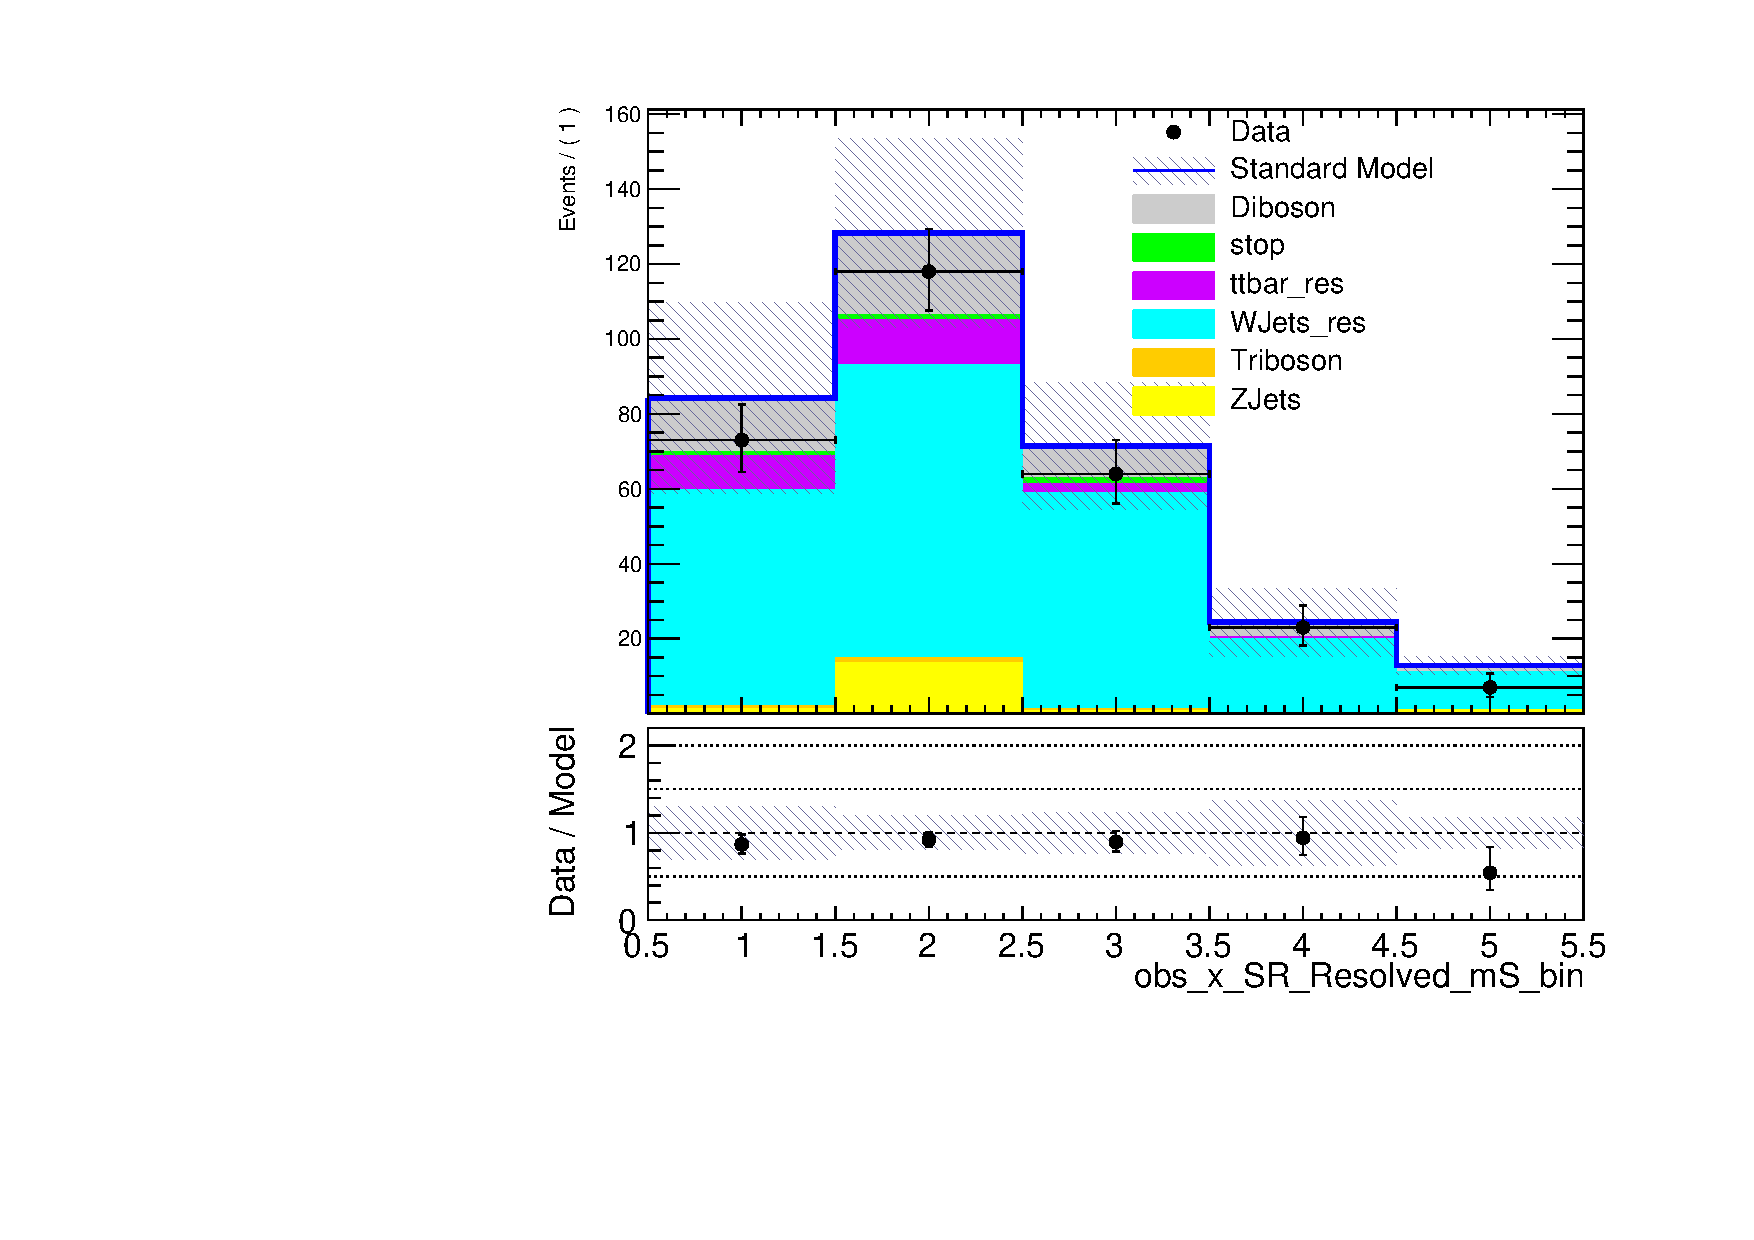
\includegraphics[width=\textwidth]{figures/12_results/BkgOnly/SR_Resolved_mS_bin_afterFit.pdf}
    \caption{\resolved SR post-fit}\label{fig:postfit_resolved_SR_bkgonly}
  \end{subfigure} \\ \vspace{1em}
  \begin{subfigure}{0.45\textwidth}
    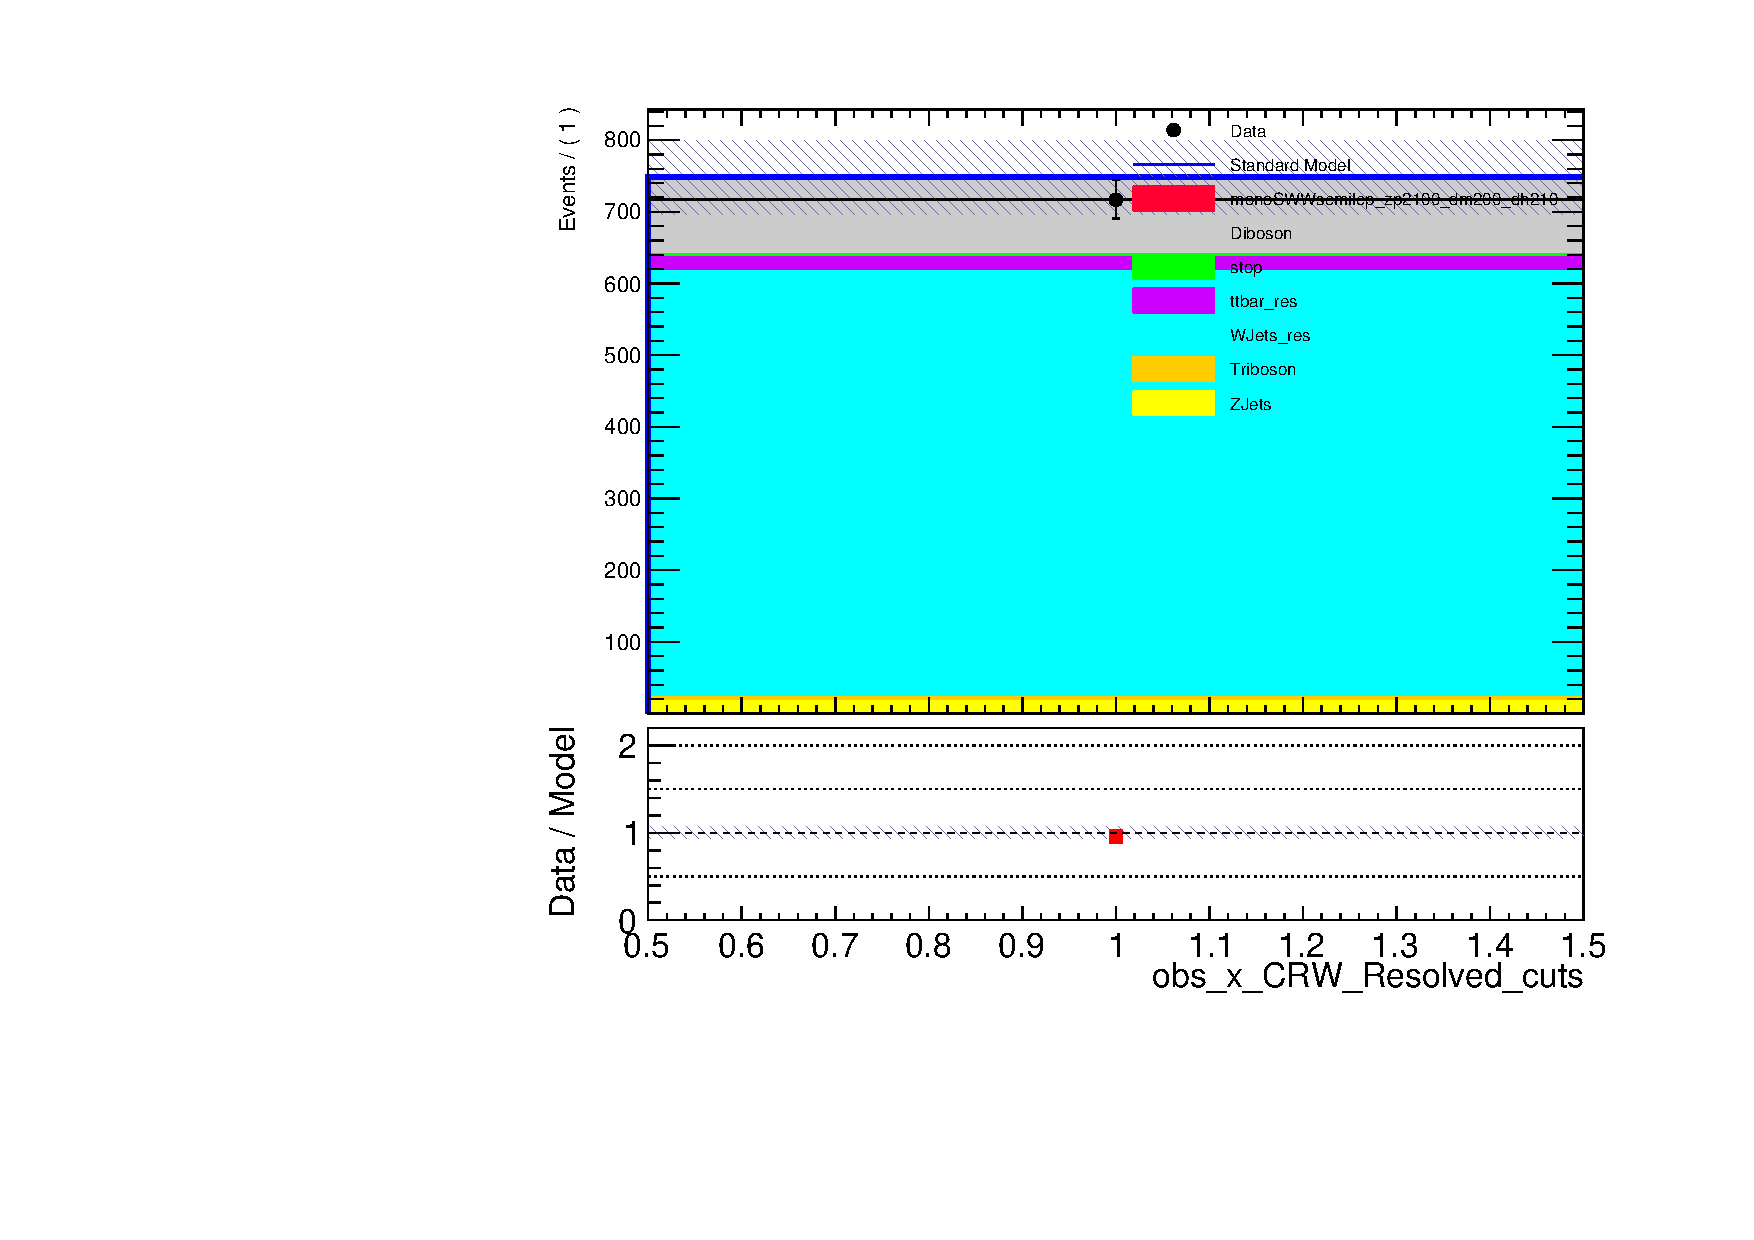
\includegraphics[width=\textwidth]{figures/12_results/BkgOnly/CRW_Resolved_cuts_beforeFit.pdf}
    \caption{\resolved CRW pre-fit}\label{fig:prefit_resolved_CRW_bkgonly}
  \end{subfigure} \hspace{1em}
  \begin{subfigure}{0.45\textwidth}
    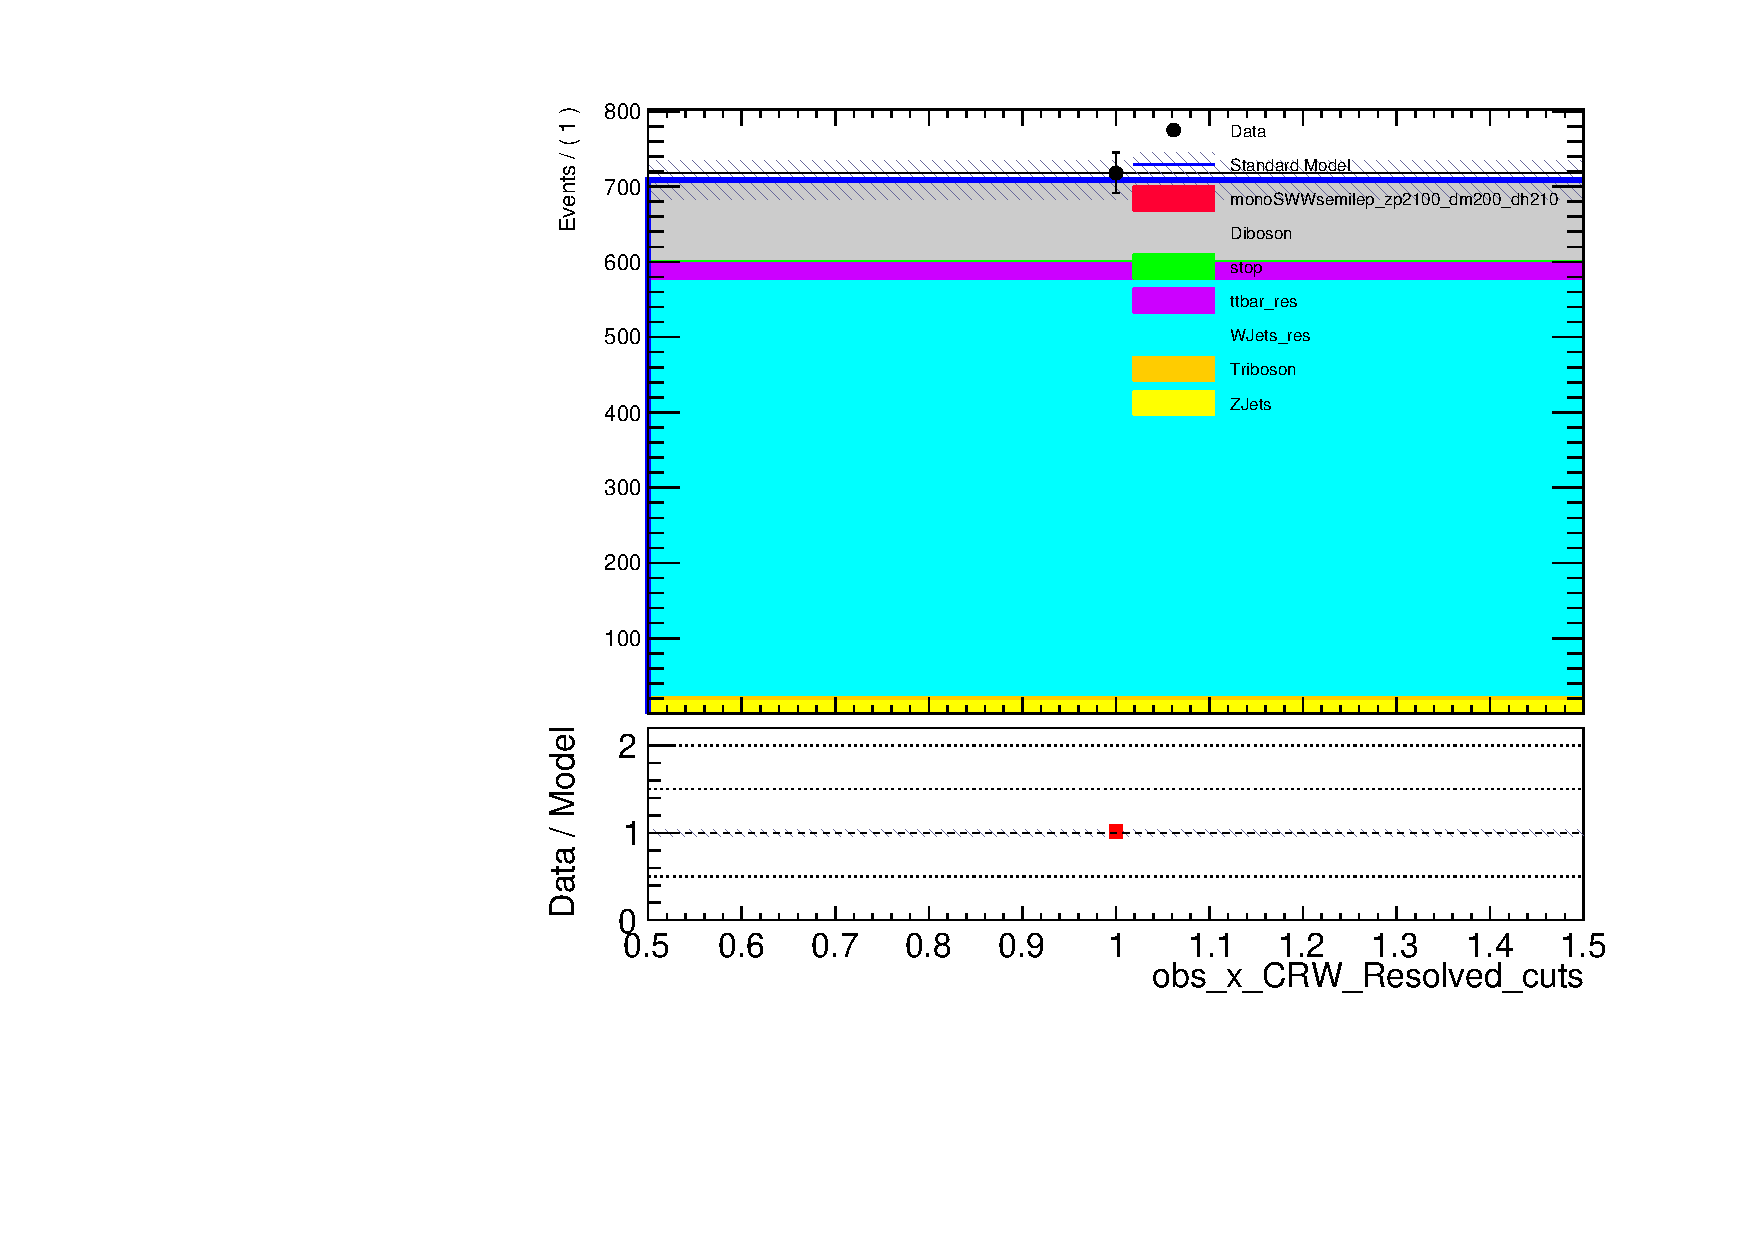
\includegraphics[width=\textwidth]{figures/12_results/BkgOnly/CRW_Resolved_cuts_afterFit.pdf}
    \caption{\resolved CRW post-fit}\label{fig:postfit_resolved_CRW_bkgonly}
  \end{subfigure} \\ \vspace{1em}
    \begin{subfigure}{0.45\textwidth}
    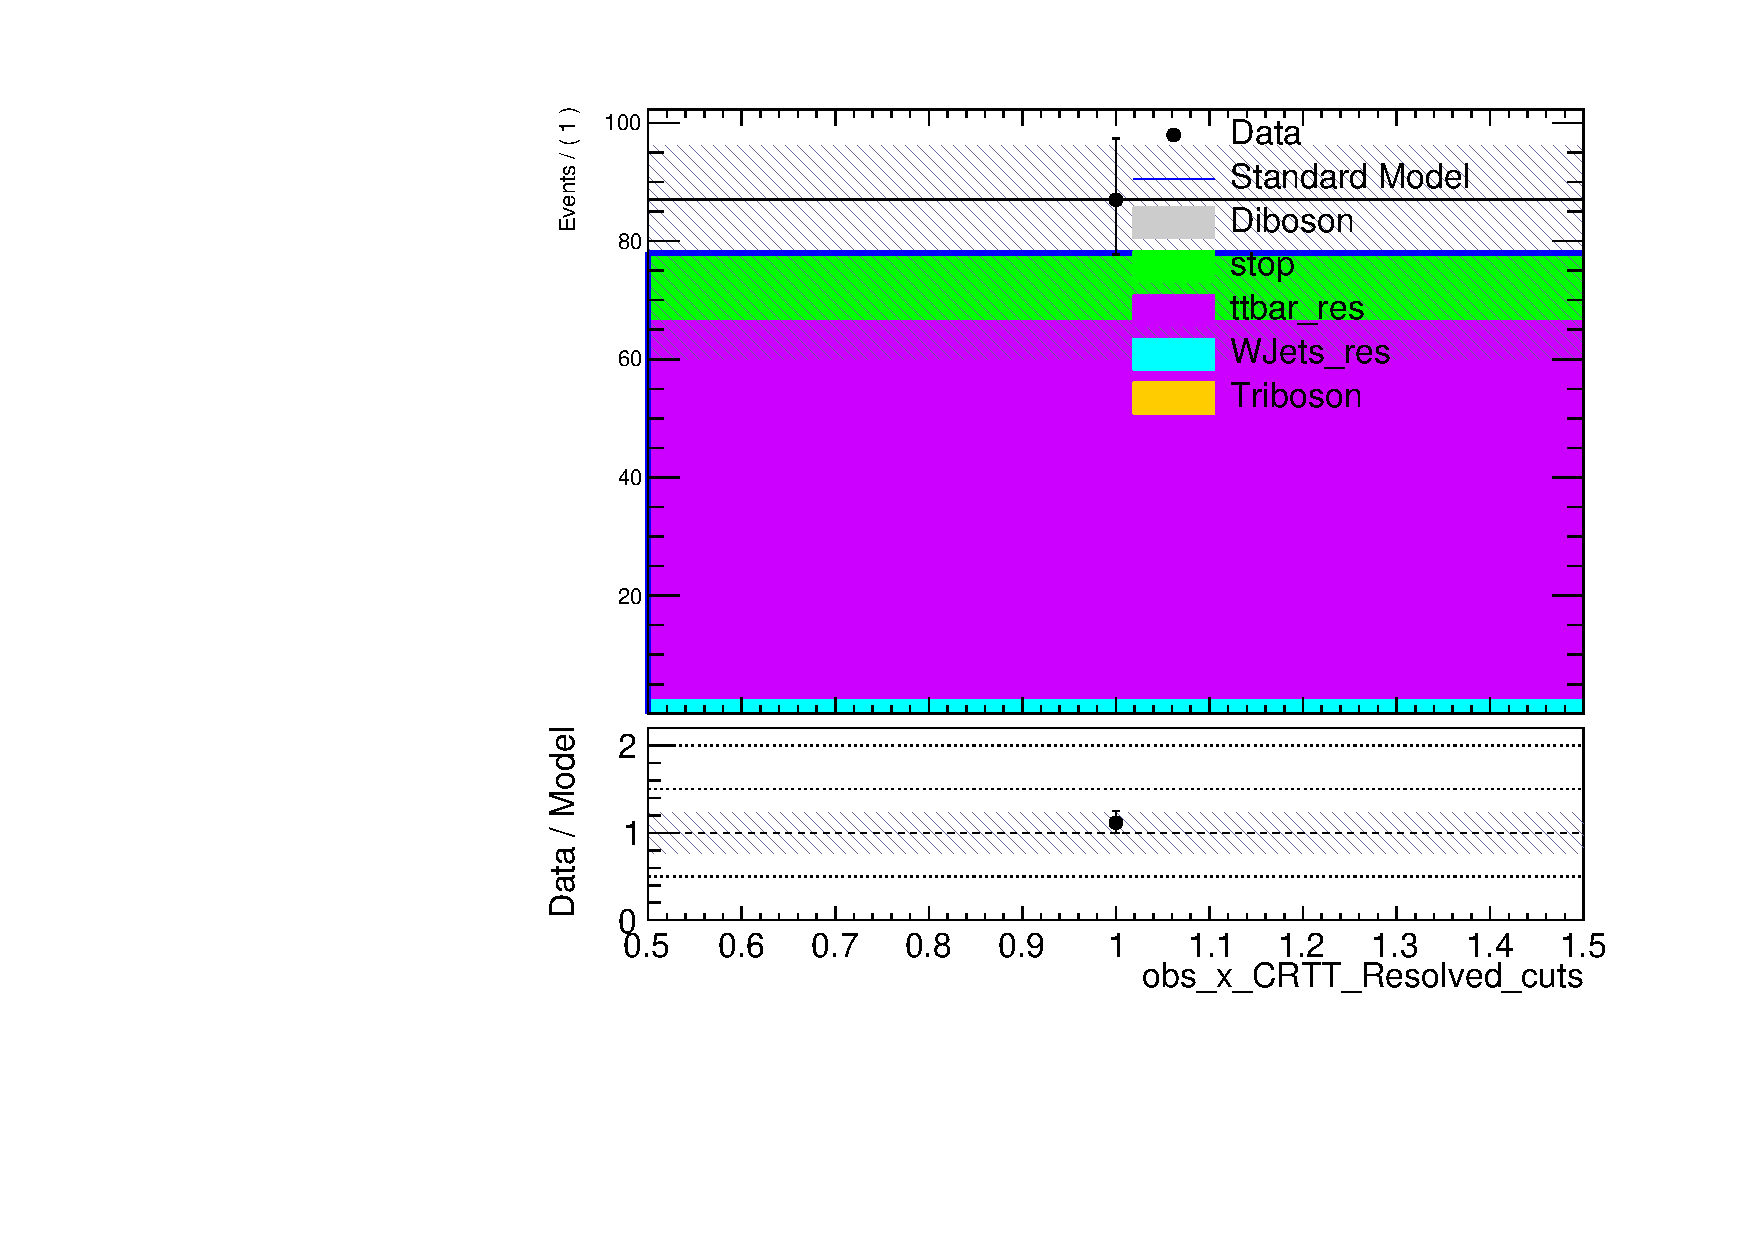
\includegraphics[width=\textwidth]{figures/12_results/BkgOnly/CRTT_Resolved_cuts_beforeFit.pdf}
    \caption{\resolved CRTT pre-fit}\label{fig:prefit_resolved_CRTT_bkgonly}
  \end{subfigure} \hspace{1em}
  \begin{subfigure}{0.45\textwidth}
    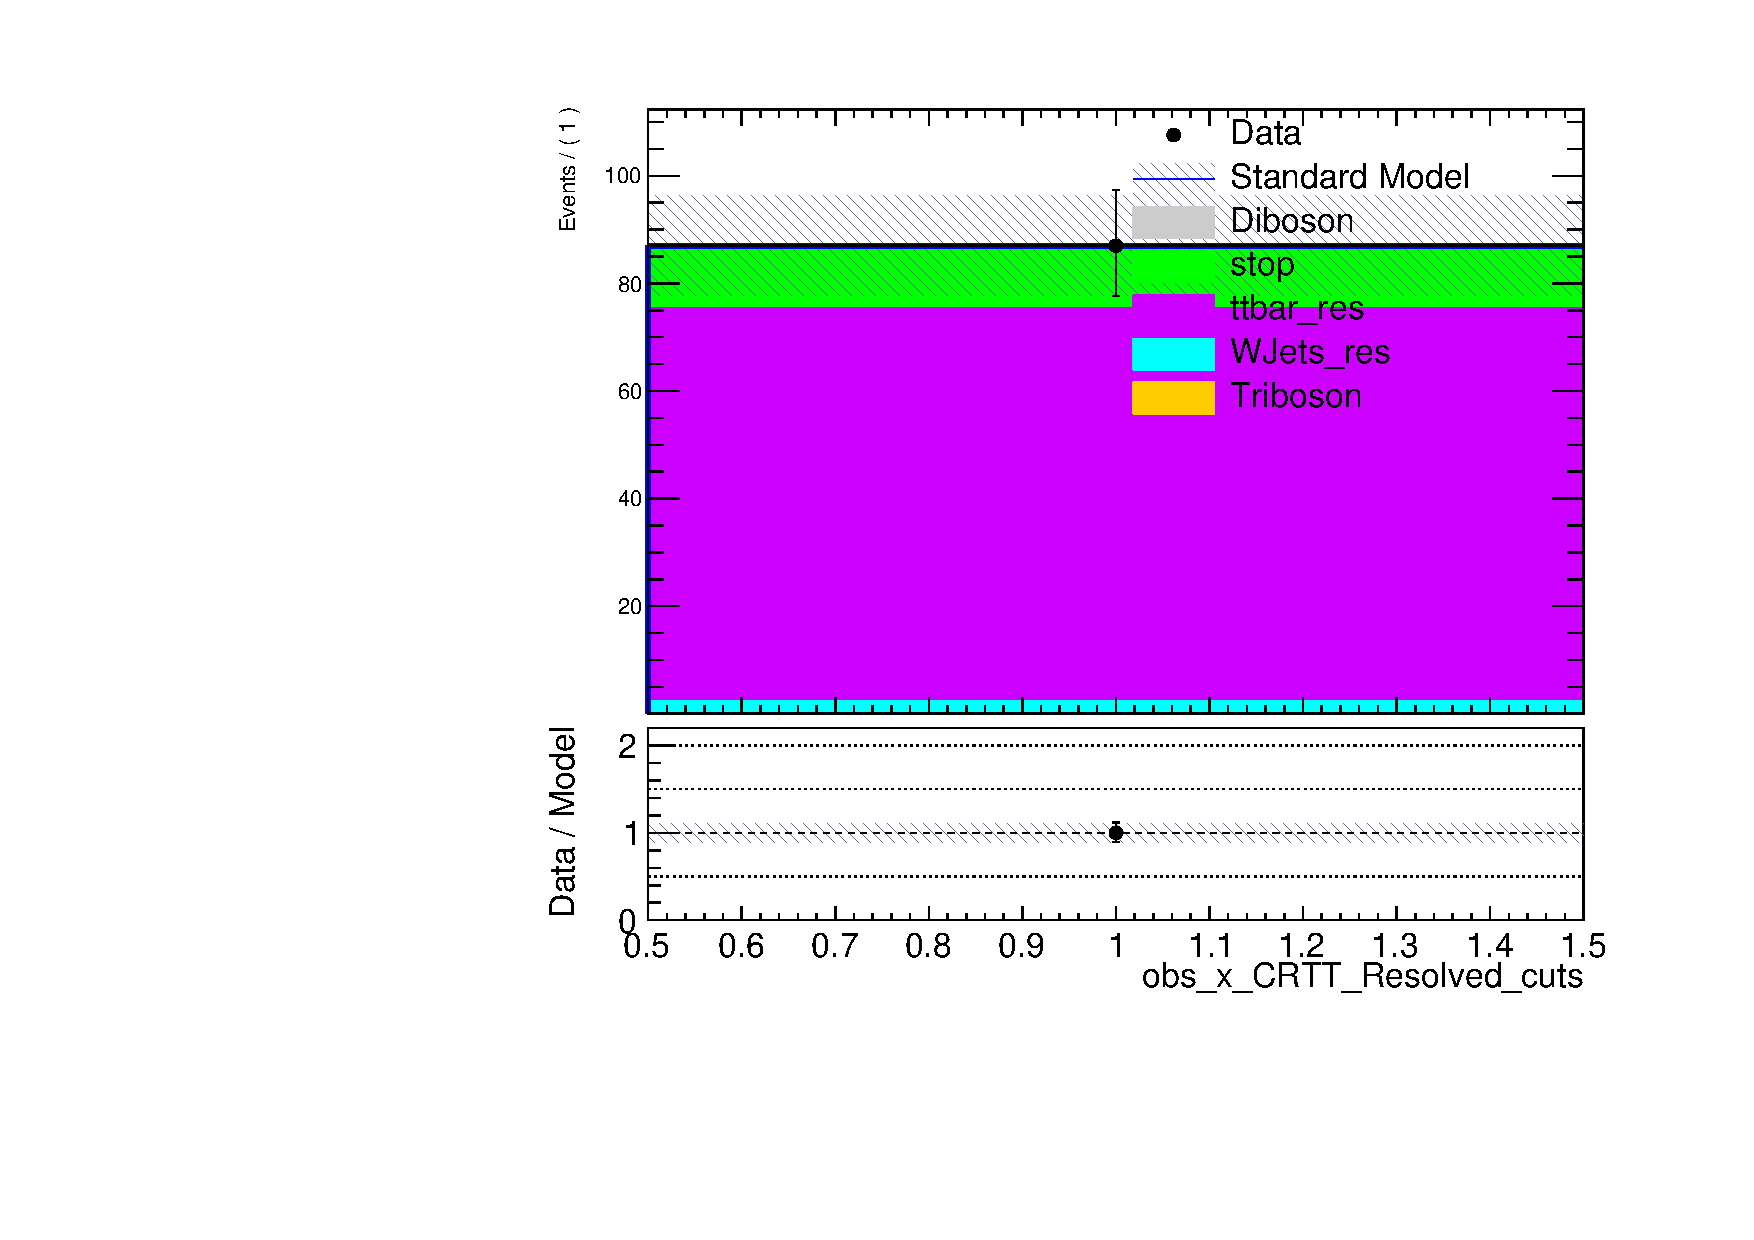
\includegraphics[width=\textwidth]{figures/12_results/BkgOnly/CRTT_Resolved_cuts_afterFit.pdf}
    \caption{\resolved CRTT post-fit}\label{fig:postfit_resolved_CRTT_bkgonly}
  \end{subfigure}
  \caption[Pre- and post-fit distributions in \resolved analysis regions for background-only fit]{Pre-fit (left) and post-fit (right) distributions for a background-only fit in the three \resolved analysis regions, with the binning used in the HistFitter fit. The Run-2 data set is used in the control regions and Asimov data is used in the signal regions. Background MC is normalized to the data luminosity of \Lumi.}
  \label{fig:pre_post_resolved_bkgonly}
\end{figure}

\subsection{Nuisance Parameter Pulls and Correlations}

\section{Comparison of SM Background Expectation and Data in the Signal Region}

\section{Exclusion of the Dark Higgs Signal Model}

\subsection{Signal+Background Fit}

\subsubsection{Nuisance Parameter Pulls and Correlations}

\subsubsection{Ranking of Systematic Uncertainties}

\subsection{Hypothesis Testing and Model Exclusion}

\begin{figure}[h]
  \centering
  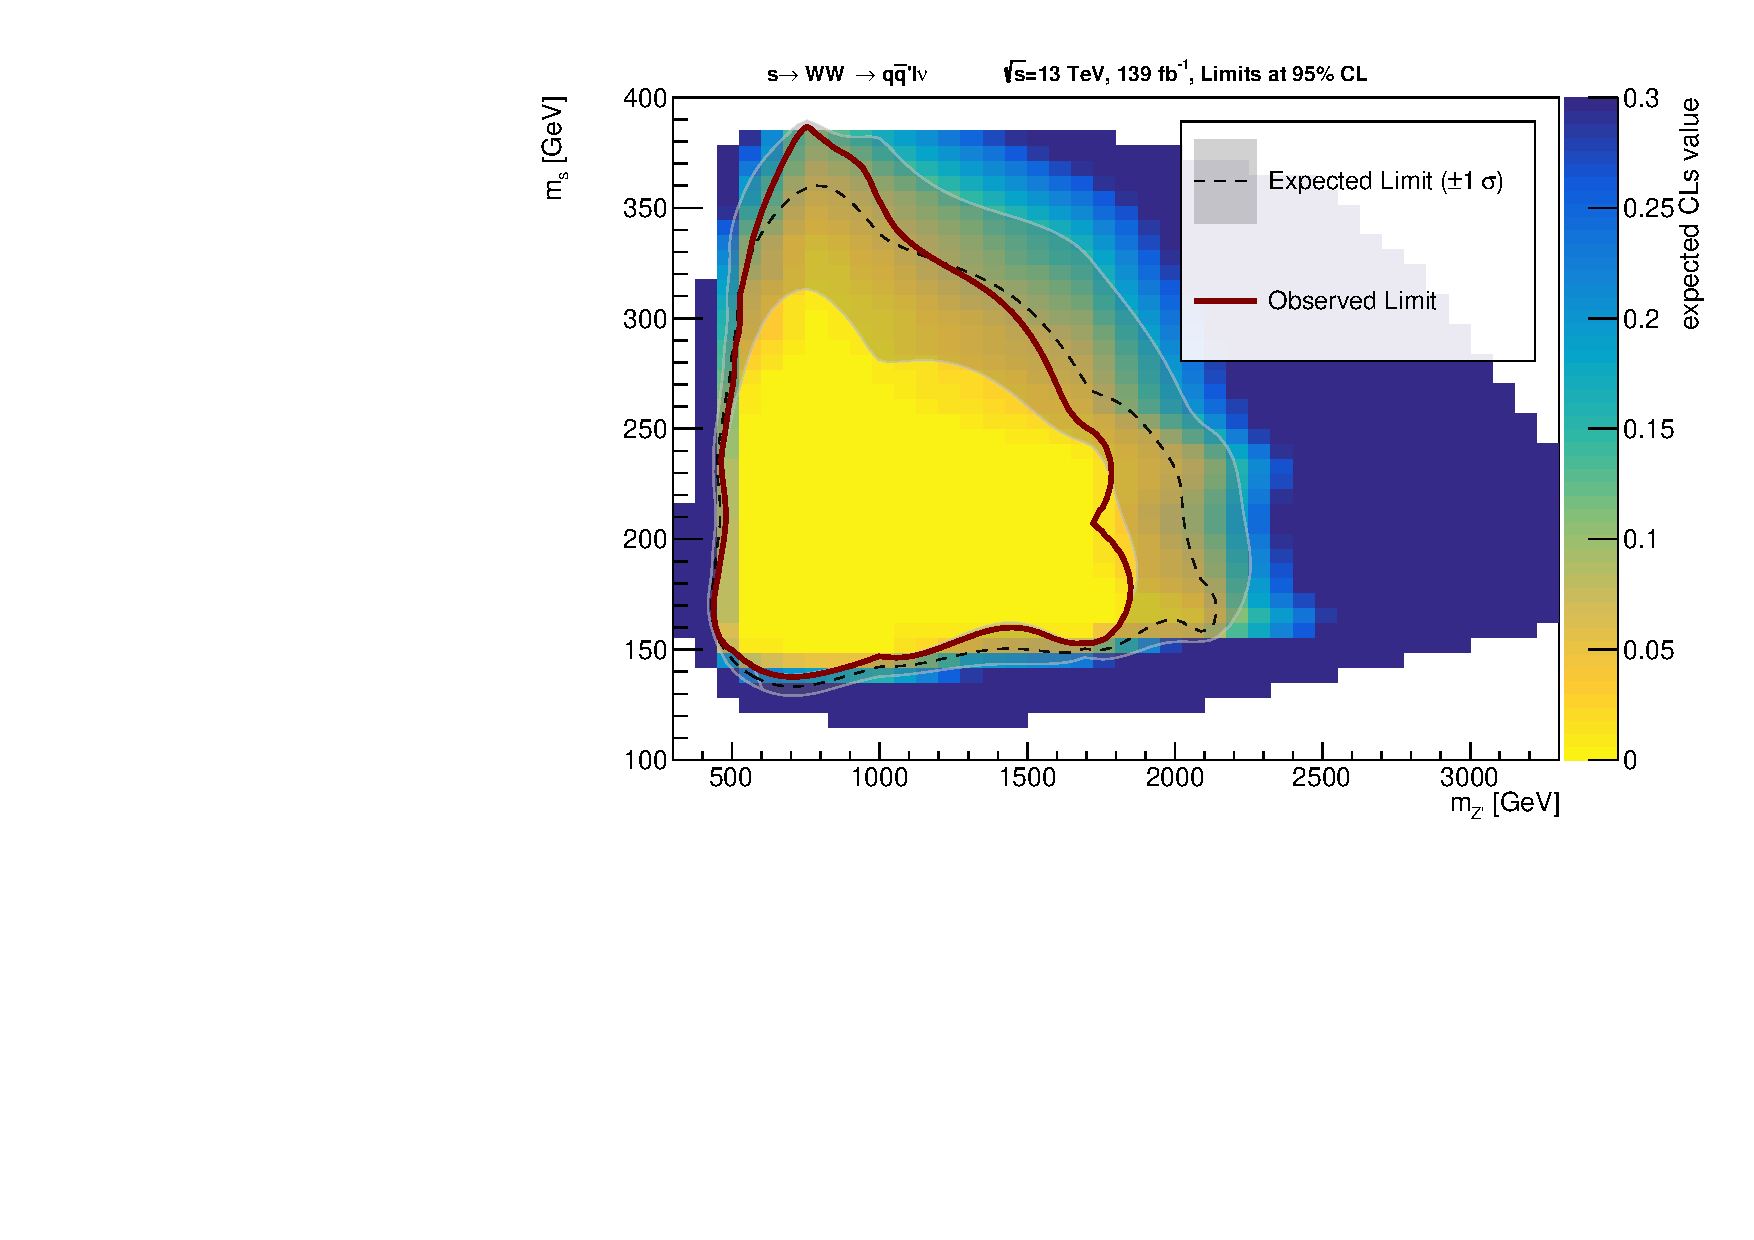
\includegraphics[width=0.8\textwidth]{Figures/8/unblinded_nosig.pdf}
  \caption[]{Projected (grey dashed with \(\pm1\sigma\) uncertainty band) and observed (solid red) range of \ms and \mZp in the DH model excluded by this search. All \ms and \mZp contained within the solid red line are excluded by the search for the choice of \(\sin\theta=0.01\), \(\gchi=1.0\) and \(g_q=0.25\).}
  \label{fig:limits}
\end{figure}

\begin{figure}[h]
  \centering
  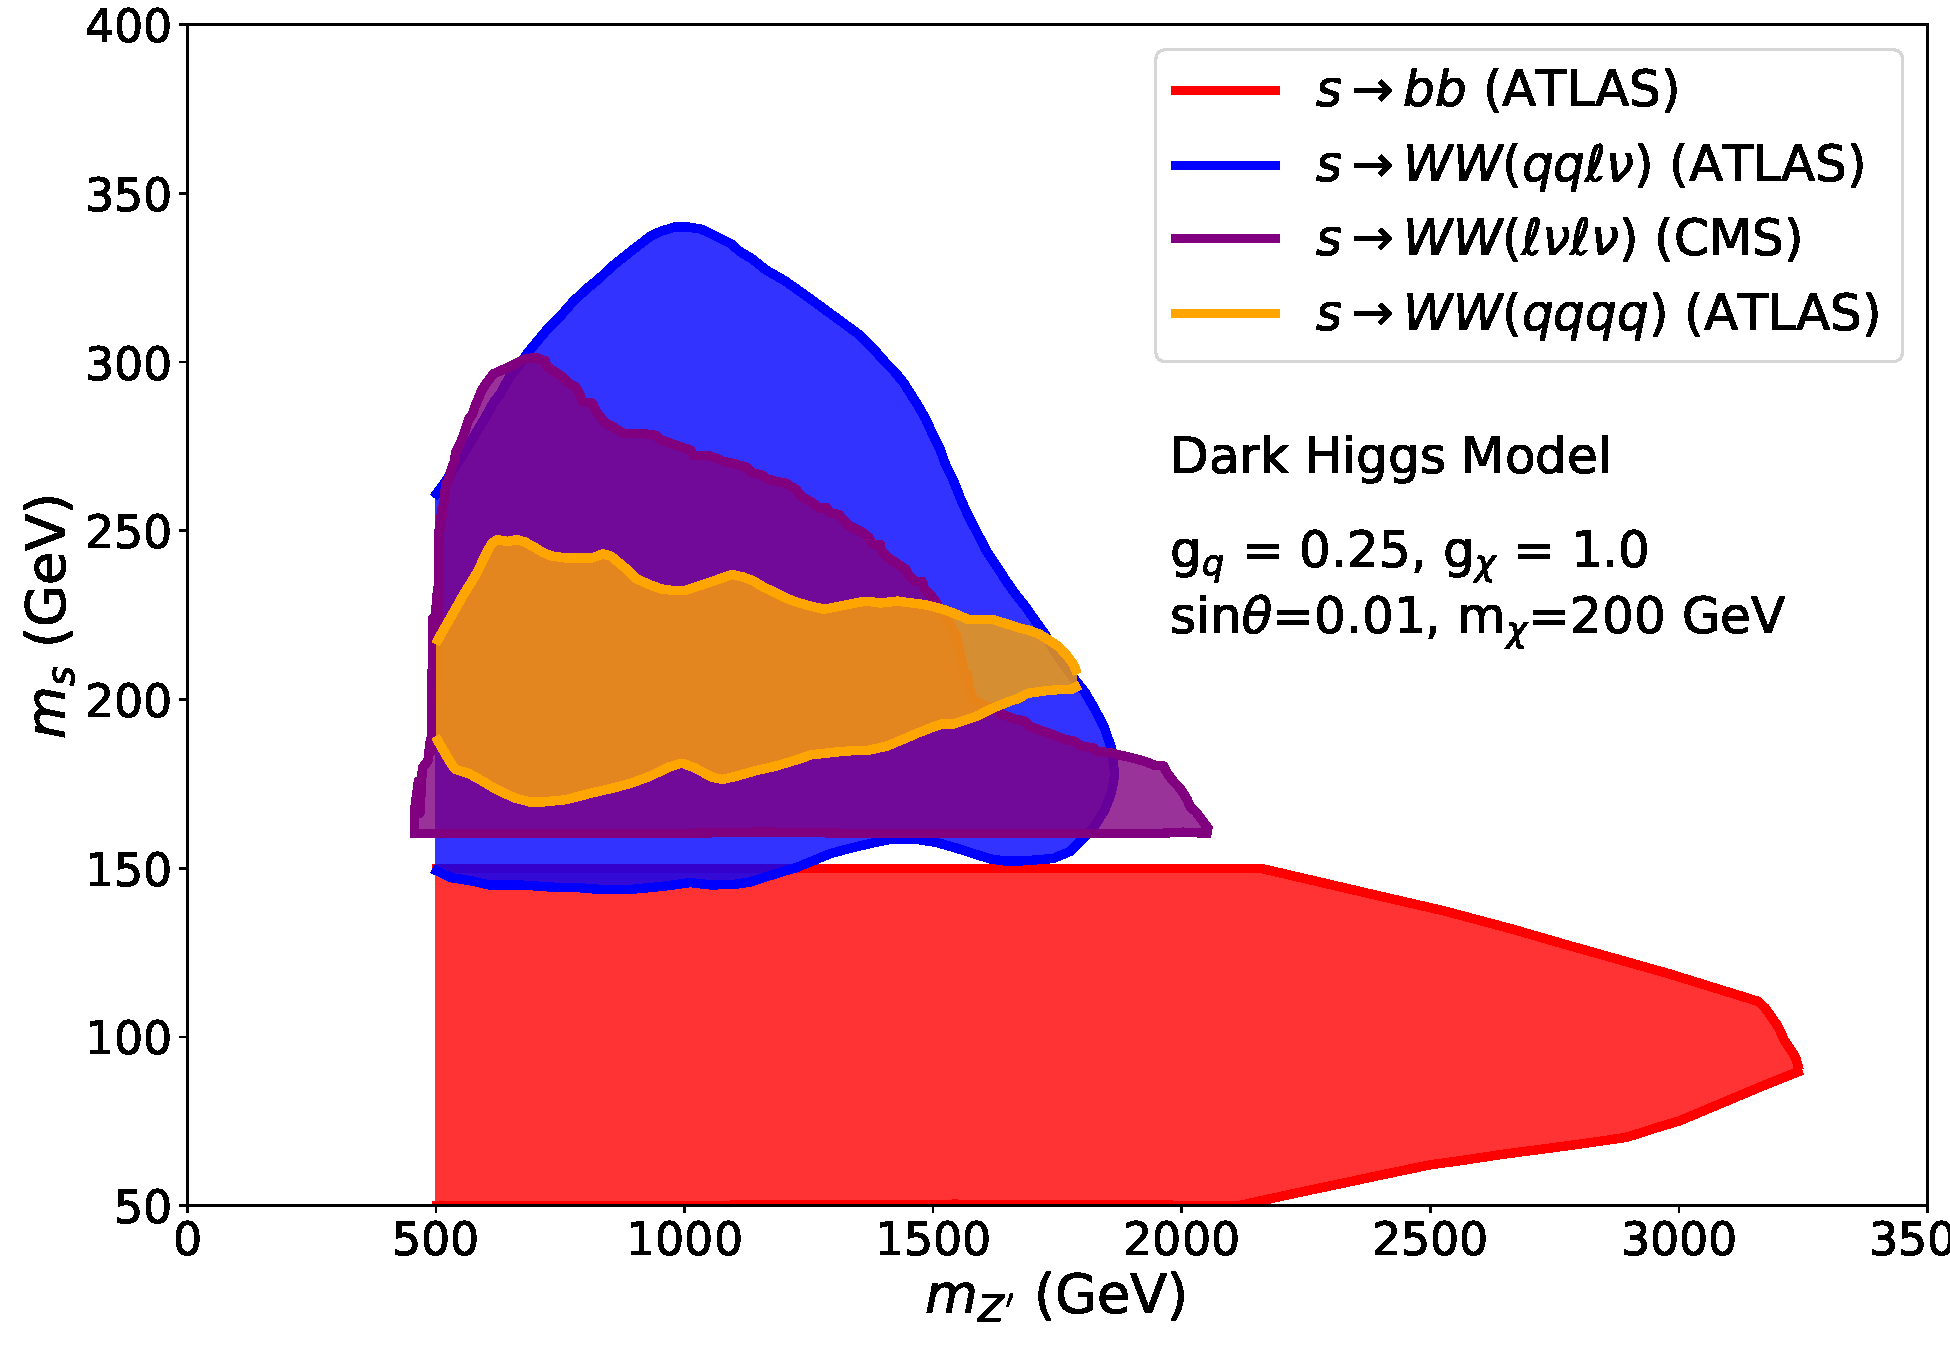
\includegraphics[width=0.8\textwidth]{Figures/8/combined_contour.pdf}
  \caption[]{Summary of \ms and \mZp parameters in the Dark Higgs model excluded by all searches for the model by ATLAS and CMS. All values of \ms and \mZp contained within a coloured area are excluded. The range excluded by the search presented in this thesis is shown in blue.}
  \label{fig:limits_comparison}
\end{figure}


